First task of utilizing a membrane-in-the-middle system, for doing cavity optomechanics, is to build a cavity and measure its properties before complicating things, by putting a membrane inside it. Our Fabry-Perot cavity (in all its simplicity), consists of a flat bottom mirror and a curved top mirror, which is the in-coupling mirror. This is a stable configuration if the radius of curvature of the curved mirror is larger than the cavity length $R > L$, which is satisfied in our case since $R = 2.5$ \SI{}{\centi\meter} and the cavity length is $L \sim 1.5$ \SI{}{\milli\meter}. The waist of the beam (radius) $w_0 \sim$ \SI{40}{\micro\meter} is placed at the flat mirror by a movable lens of focal length $f = 11$ \SI{}{\milli\meter}. For a desired distance to the bottom mirror, this condition mode matches the wavefront curvature to the mirrors curvature at wavelength $\lambda = 850$ \SI{}{\nano\meter} according to basic Gaussian optics see figure \ref{fig:bare_cavity}. The free spectral range of the cavity is $100$ \SI{}{\giga\hertz}. The rather short cavity length is chosen to increase the coupling $G = \frac{\omega_c}{L}$ as much as possible. The spot size $w_0$ is another important parameter, since we want to resolve the membrane mode shapes $\frac{L_m}{n} > w_0$, where $L_m$ is the side length of the membrane and $n$ is the highest mode number. Not being deeply in this regime results in a decreased coupling, because of the overlap integral between mechanical mode and spot size.

\begin{figure}[h]
\centering
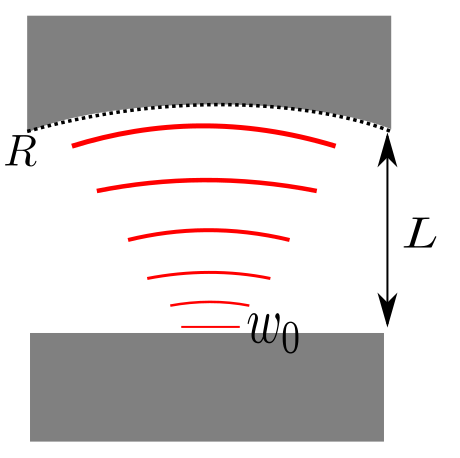
\includegraphics[scale=0.5]{cavity.png}
\caption{Bare cavity design.}
\label{fig:bare_cavity}
\end{figure}

We measure our bare cavity linewidth at \SI{852}{\nano\meter} to be roughly \SI{0.5}{\mega\hertz} as shown from the trace in figure \ref{fig:bare_cavity_linewidth}\footnote{$\kappa$ in the figure is actually $\kappa/2\pi$}. The axis is calibrated using EOM generated sidebands at \SI{3}{\mega\hertz} and the cavity linewidth $\kappa/2\pi$ is obtained by a Lorentzian fit.

\begin{figure}[h]
\centering
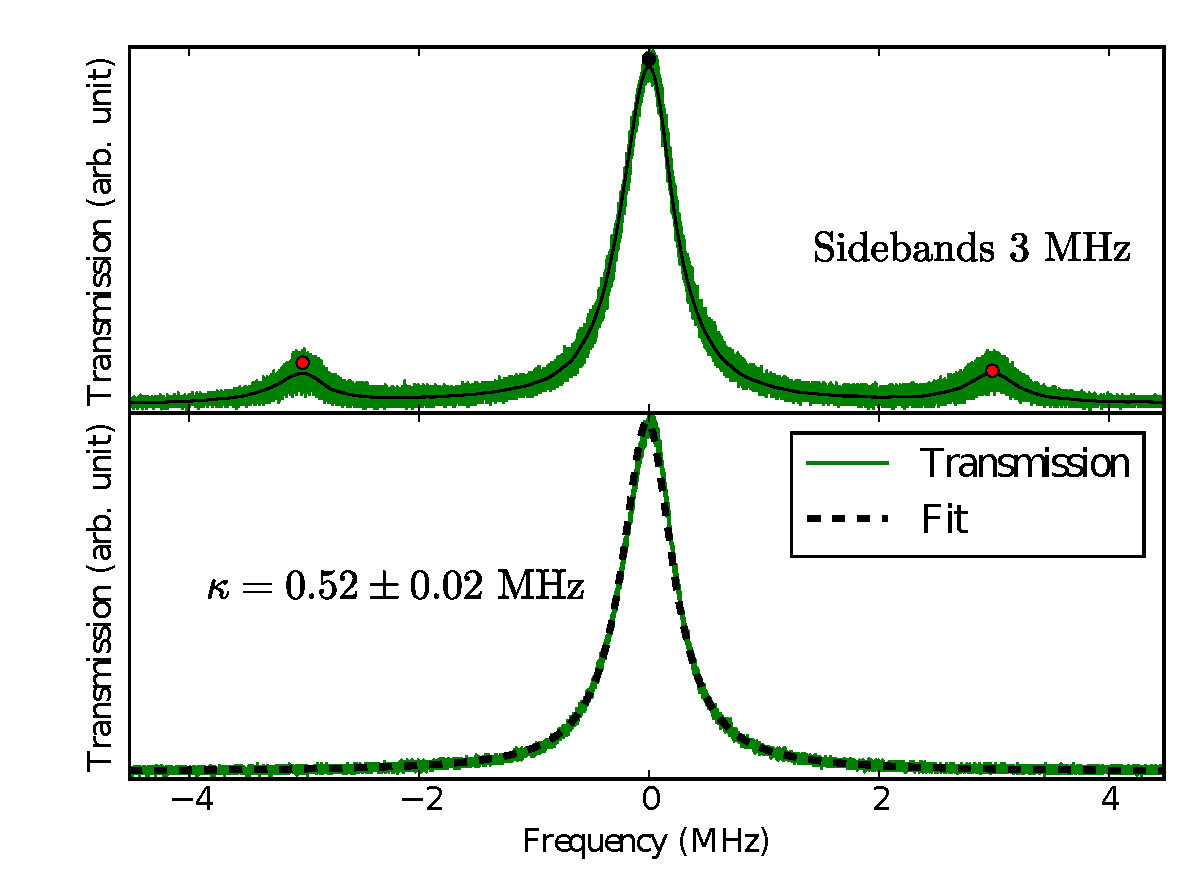
\includegraphics[scale=0.7]{cavity_linewidth.pdf}
\caption{Bare cavity linewidth measured by calibrating the frequency axis using sidebands.}
\label{fig:bare_cavity_linewidth}
\end{figure}

The bare cavity free spectral range is measured to be \SI{84.9}{\giga\hertz} see appendix \ref{sec:bare_fsr}. The assembled bare cavity is a bit longer than initially intended, but the added length can be assigned to the curvature of one of the mirrors. Our measured cavity finesse is then roughly 163000, which is a high finesse for optical cavities.